\documentclass{article}
\usepackage[margin=6cm]{geometry}
\usepackage{tikz}
\usepackage{xspace}
\def\pdfxup{\texttt{pdfxup}\xspace}

\begin{document}
\title{\pdfxup \\[2mm]
  \normalsize
  version 2.12 -- 2024/06/11}
\author{Nicolas Markey}
\date{}

\maketitle

\def\abstractname{}
\begin{abstract}
\pdfxup is a shell script that creates $n$-up PDF documents, while at
the same time removing as much white stripes as possible. This
document reviews the main features of \pdfxup. See the \verb+man+ page
for more details.
\end{abstract}

\section{Basic usage}
Running \pdfxup with no options creates a 2-up document from the
original PDF file:
\begin{center}
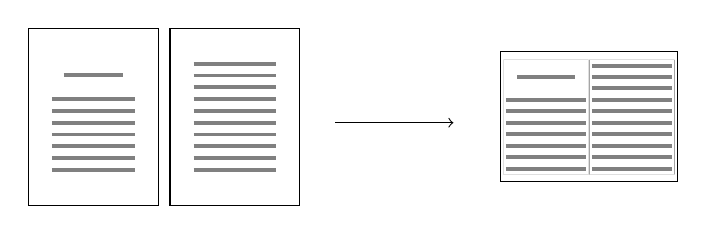
\begin{tikzpicture}[scale=1.5]
  \begin{scope}
  \draw (0,0) |- (1.1,1.5) |- cycle;
  \foreach \x in {.3,.4,...,.9}
           {\draw [line width=.5mm,black!50!white] (.2,\x) -- +(.7,0);}
  \draw [line width=.5mm,black!50!white] (.3,1.1) -- +(.5,0);
  \end{scope}
  \begin{scope}[xshift=1.2cm]
  \draw (0,0) |- (1.1,1.5) |- cycle;
  \foreach \x in {.3,.4,...,1.2}
           {\draw [line width=.5mm,black!50!white] (.2,\x) -- +(.7,0);}
  %\draw [line width=.5mm,black!50!white] (.3,1.2) -- +(.4,0);
  \end{scope}
  %
  \draw[->] (2.6,.7) -- +(1,0);% node[midway,above] {scale=97\%};
  %
  \begin{scope}[yshift=2mm,xshift=4cm]
    \draw (0,0) |- (1.5,1.1) |- cycle;    
    \begin{scope}[yshift=-1.8mm,xshift=-1.5mm,scale=.97]
      \draw[line width=.02pt] (.178,.25) |- (.922,1.25) |- cycle;
      \foreach \x in {.3,.4,...,.9}
             {\draw [line width=.5mm,black!50!white] (.2,\x) -- +(.7,0);}
      \draw [line width=.5mm,black!50!white] (.3,1.1) -- +(.5,0);
      \begin{scope}[xshift=7.5mm]
        \draw[line width=.02pt] (.178,.25) |- (.922,1.25) |- cycle;
        \foreach \x in {.3,.4,...,1.2}
           {\draw [line width=.5mm,black!50!white] (.2,\x) -- +(.7,0);}
      \end{scope}
    \end{scope}
  \end{scope}
\end{tikzpicture}
\end{center}

It removes white strips around text, so that it does not need to scale
down the original document too much. All margins in the resulting PDF
can be adapted using various options. The number of rows and columns
of pages can be modified using options \verb+-x+ and \verb+-y+. By
default, the output file is in landscape mode, but this can be changed
using option \verb+-l=no+.

Computing the boundig box is performed automatically using
GhostScript. This may take time for long documents, but it is often
sufficient to compute the bounding box on the first few pages, using
option \verb+-bb+. Bounding-box computation can be turned off (so that
original margins are kept) using \verb+-kbb+. 

It is possible to only include a subset of pages using option
\verb+-p+ (notice that if a page is listed twice, it will be included
twice).

\section{Creating a booklet}
\pdfxup can create booklets: this is similar to the operation above,
but the pages are ordered and oriented in the adequate way. Booklet
mode is triggered with the \verb+-b+ option.
\begin{center}
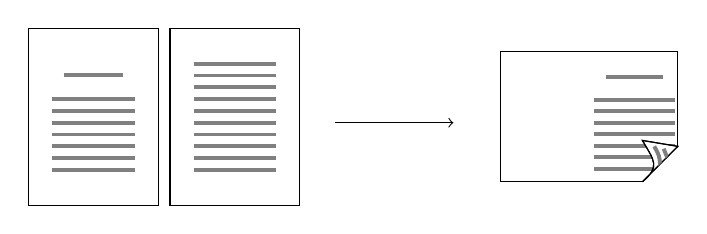
\begin{tikzpicture}[scale=1.5]
  \begin{scope}
  \draw (0,0) |- (1.1,1.5) |- cycle;
  \foreach \x in {.3,.4,...,.9}
           {\draw [line width=.5mm,black!50!white] (.2,\x) -- +(.7,0);}
  \draw [line width=.5mm,black!50!white] (.3,1.1) -- +(.5,0);
  \end{scope}
  \begin{scope}[xshift=1.2cm]
  \draw (0,0) |- (1.1,1.5) |- cycle;
  \foreach \x in {.3,.4,...,1.2}
           {\draw [line width=.5mm,black!50!white] (.2,\x) -- +(.7,0);}
  %\draw [line width=.5mm,black!50!white] (.3,1.2) -- +(.4,0);
  \end{scope}
  %
  \draw[->] (2.6,.7) -- +(1,0);% node[midway,above] {scale=97\%};
  %
  \begin{scope}[yshift=2mm,xshift=4cm]
    \draw (0,0) |- (1.5,1.1) |- cycle;    
    \begin{scope}[yshift=-1.8mm,xshift=6mm,scale=.97]
%      \draw[line width=.02pt] (.178,.25) |- (.922,1.25) |- cycle;
      \foreach \x in {.3,.4,...,.9}
             {\draw [line width=.5mm,black!50!white] (.2,\x) -- +(.7,0);}
      \draw [line width=.5mm,black!50!white] (.3,1.1) -- +(.5,0);
    \end{scope}
      \fill[white] (1.2,-.01) -| (1.51,.3) -- cycle;
      \draw[fill=white] (1.2,0) .. controls +(40:2mm) and +(-60:2mm) .. (1.2,.35) -- (1.5,.3) -- cycle;
      \begin{scope}
        \draw[clip] (1.2,0) .. controls +(40:2mm) and +(-60:2mm) .. (1.2,.35) -- (1.5,.3) -- cycle;
        \draw[line width=.5mm,black!50!white] (1.3,.3) .. controls +(-60:1mm) and +(90:2mm) ..  ++(-80:3mm);
        \draw[line width=.5mm,black!50!white] (1.38,.28) .. controls +(-69:1mm) and +(90:2mm) ..  ++(-80:3mm);
      \end{scope}
  \end{scope}
\end{tikzpicture}
\end{center}

\section{Watermarking}
Using option \verb+-w+, you can add watermarking to the original file:
\begin{center}
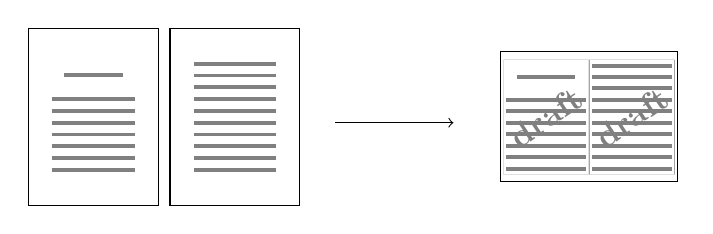
\begin{tikzpicture}[scale=1.5]
  \begin{scope}
  \draw (0,0) |- (1.1,1.5) |- cycle;
  \foreach \x in {.3,.4,...,.9}
           {\draw [line width=.5mm,black!50!white] (.2,\x) -- +(.7,0);}
  \draw [line width=.5mm,black!50!white] (.3,1.1) -- +(.5,0);
  \end{scope}
  \begin{scope}[xshift=1.2cm]
  \draw (0,0) |- (1.1,1.5) |- cycle;
  \foreach \x in {.3,.4,...,1.2}
           {\draw [line width=.5mm,black!50!white] (.2,\x) -- +(.7,0);}
  %\draw [line width=.5mm,black!50!white] (.3,1.2) -- +(.4,0);
  \end{scope}
  %
  \draw[->] (2.6,.7) -- +(1,0);% node[midway,above] {scale=97\%};
  %
  \begin{scope}[yshift=2mm,xshift=4cm]
    \draw (0,0) |- (1.5,1.1) |- cycle;    
    \begin{scope}[yshift=-1.8mm,xshift=-1.5mm,scale=.97]
      \path (.178,.5) -- (.922,1) node[midway,sloped,opacity=.5]
            {\bfseries\large draft};
      \draw[line width=.02pt] (.178,.25) |- (.922,1.25) |- cycle;
      \foreach \x in {.3,.4,...,.9}
             {\draw [line width=.5mm,black!50!white] (.2,\x) -- +(.7,0);}
      \draw [line width=.5mm,black!50!white] (.3,1.1) -- +(.5,0);
      \begin{scope}[xshift=7.5mm]
      \path (.178,.5) -- (.922,1) node[midway,sloped,opacity=.5]
            {\bfseries\large draft};
        \draw[line width=.02pt] (.178,.25) |- (.922,1.25) |- cycle;
        \foreach \x in {.3,.4,...,1.2}
           {\draw [line width=.5mm,black!50!white] (.2,\x) -- +(.7,0);}
      \end{scope}
    \end{scope}
  \end{scope}
\end{tikzpicture}
\end{center}


\pdfxup has many other options, setting up margins, frames, order of pages,~...
Please look at the \texttt{man} page for more details.


\end{document}
